\documentclass[12pt, a4paper]{article} 
 
\usepackage[utf8]{inputenc}
 

\usepackage[bottom = 8em]{geometry} % to change the page dimensions
\geometry{a4paper} % or letterpaper (US) or a5paper or....
 
\usepackage{graphicx} % support the \includegraphics command and options
 
\usepackage{booktabs} % for much better looking tables
\usepackage{array} % for better arrays (eg matrices) in maths
\usepackage{float}
\usepackage{paralist} % very flexible & customisable lists (eg. enumerate/itemize, etc.)
\usepackage{verbatim} % adds environment for commenting out blocks of text & for better verbatim
\usepackage{subfig} % make it possible to include more than one captioned figure/table in a single float
% These packages are all incorporated in the memoir class to one degree or another...
 
 
 
\usepackage{amsmath, amssymb}% for mathematical symbols
\usepackage[colorlinks=true,linkcolor=black]{hyperref} % for hyperreferences with black color
%\usepackage[T1]{fontenc} % Uncomment for norwegian document
%\usepackage[norsk]{babel} %
 
%%% HEADERS & FOOTERS
\usepackage{fancyhdr} % This should be set AFTER setting up the page geometry
\pagestyle{fancy} % options: empty , plain , fancy
\renewcommand{\headrulewidth}{0pt} % customise the layout...
\lhead{}\chead{}\rhead{}
\lfoot{}\cfoot{\thepage}\rfoot{}

 
%%% SECTION TITLE APPEARANCE
\usepackage{sectsty}
\allsectionsfont{\sffamily\mdseries\upshape} % (See the fntguide.pdf for font help)
% (This matches ConTeXt defaults)
 
%%% ToC (table of contents) APPEARANCE
\usepackage[nottoc,notlof,notlot]{tocbibind} % Put the bibliography in the ToC
\usepackage[titles,subfigure]{tocloft} % Alter the style of the Table of Contents
\renewcommand{\cftsecfont}{\rmfamily\mdseries\upshape}
\renewcommand{\cftsecpagefont}{\rmfamily\mdseries\upshape} % No bold!
 
 
%%% END Article customizations
 
%%% The "real" document content comes below...
 
\title{AI prog 1}
\author{Eivind Hærum \& \ Hong-Dang Lam}
\date{\today} % Activate to display a given date or no date (if empty),
         % otherwise the current date is printed 
 
\begin{document}
\maketitle
%\begin{abstract}
% 
%Abstract
% 
%\end{abstract}
 
\newpage
\tableofcontents
\newpage
 
\section{Demo}
Please refer to the delivered code.

\section{Our implementation}

\subsection{The internal representation}
We have a Board class to maintain a working gameboard which contains a 2 dimensional array to represent our board, and a 1 dimensional array to represent the remaining pieces. We also have numerous fields and arrays to act as counters for how many Pieces are placed on a given row f.ex. and to check whether a board is internal or not(internal meaning a temporary board used in either novice or minimax)\\ \\
The game appears like this whenever a move is made:\\
\begin{figure}[H]
\begin{verbatim}

Turn 0 minimax_3
choose piece:
1
Chosen piece: 1: (r*)
 .   .   .  (r*)
 .   .   .   . 
 .   .   .   . 
 .   .   .   . 

Remaining:
 0:(r)   2:(R)   3:(R*)  4:|r|    5:|r*|  6:|R|  7:|R*|  8:(b)  9:(b*)  
10:(B)  11:(B*) 12:|b|  13:|b*|  14:|B|  15:|B*|  
____________________________________________________________

Turn 1 human
Chosen piece: 4: |r|
choose an X, and Y
\end{verbatim}
\caption{Initial move}
\label{figure1}
\end{figure}
\noindent
And this is how it looks after a few moves have been played (and coincidentally where the minimax bot will win no matter what piece it's given):\\

\begin{figure}[H]
\begin{verbatim}

Turn 7 human
Chosen piece: 0: (r)
choose an X, and Y
1 3
|r|   .   .   (r*)
|B*|  .  (B*) (R*)
 .    .   .    . 
|b*| (r) (b)   . 

Remaining:
2:(R)  5:|r*|  6:|R|  7:|R*|  9:(b*)  10:(B)  12:|b|  14:|B|  
____________________________________________________________

Turn 8 minimax_3
choose piece:
\end{verbatim}
\caption{Midgame move}
\label{figure2}
\end{figure}
\noindent
Finally a winning state looks like this:\\
\begin{figure}[H]
\begin{verbatim}

Turn 8 minimax_3
choose piece:
2
Chosen piece: 2: (R)
|r|   .   .   (r*)
|B*| (R) (B*) (R*)
 .    .   .    . 
|b*| (r) (b)   . 

Remaining:
5:|r*|  6:|R|  7:|R*|  9:(b*)  10:(B)  12:|b|  14:|B|  
____________________________________________________________

Player1 (minimax_3) won
____________________________________________________________
Stats (minimax_3 vs human):
Runs: 1
Player1 (minimax_3) wins:1
Player2 (human) wins:0
Ties:0

\end{verbatim}
\caption{Post game}
\label{figure3}
\end{figure}

\subsection{Evaluate the board}
To be able to easily check whether a given board is a final state or not we have constructed several counters. We have a 1 dimensional array with length 4 to keep track of placed pieces on each row and column, and 2 seperate fields for the diagonals. We have a few functions which utilize these properties by only checking for a winstate given that there are 4 pieces in a row on a given row/col/diagonal. If there are 4 pieces in a row and it is not a winning state we increment the counter to 5 and thus prevent the check from happening again.


\subsection{Heuristic}
The heuristic gives 500 points if a node is a winning node with depth 1 or any odd numbered depth, this means that we have recieved a Piece and placed it on the board which led to a win. If the depth is an even number however and the node is a winning state, then the heuristic gives -500, because that would mean that the opponent have just put down a piece and there's a winning state. \\
The heuristic gives points for whenever there's 2 pieces with similar property in a row/col/diagonal because that would bring it closer to a winning state, which is easier to notice for the computer, and might be harder for a human to see, therefore it considers 2 in a row to be a partially good state. The heuristic gives 2 points for every property that are 2-pieces in a row, for instance if we have a big square red piece next to a big square holed red piece the heuristic would give 6 points (2 for big, 2 for square and 2 for red).\\
The trickiest part is the 3 pieces in a row, the system tries to check whenever there's 3 pieces in a row with the same properties. If it for instance sees 3 red pieces in a row, it will start to count how many blue pieces there are left, if there are an even number of blue pieces left, it will give partial credit. This is because you will win if both players are trying to only give blue to avoid the loss, the last blue piece given will be ours, therefore it'll force the other bot to give us a red piece which will lead to a win. That's why we give partial credit for 2 pieces in a row with the same property, because this will easier lead to the 3-pieces state. The heuristic gives 5 points for every property that are 3-pieces in a row, for instance if we have a big square red piece next to a big square holed red piece and a big round red piece the heuristic would give 10 points (5 for big, 5 for red).\\
Our minimax bot doesn't really care about what specific property each piece have as long as the numbers add up, the bot checks how many pieces there are in a row then checks how many of the same properties the pieces have. This is done by making an int array of size 8, which counts number of holes, non-holes, round, square, big, small, reds and blues. It then gets an int array of size 8 which is the same as the one mentioned earlier, with each index in the array representing a property.

\subsection{Minimax with Alpha-Beta pruning}
The way our algorithm implements alpha-beta pruning is by using the well established depth-first approach to both generate and evaluate the children at depth N on the go. The aim is to only generate the needed children and only keep track of the best children, and propagate the value of an arbitrary chosen one of the best children (if there are more than one optimal one. Otherwise return the singular best state). \\ 
Thus if we have a minimax\_3 bot, it will first generate the root (the state it is in now), then generate its leftmost child (placing the provided piece in the top left available corner on the internal board), and choose the first available Piece from the remaining pieces to send to its child. Then this node generates its leftmost child and repeats the same process. Finally the process is done again, but because we are now at the maximum depth we are now at leaf level, meaning we now get to evaluate the node with the heuristic function and then propagate this value back up to the parent. \\
As we are at depth 2 we are at a Max node, thus we attempt to maximize alpha, meaning we update alpha to the returned value if it is better than the previous alpha. Because we have yet to propagate a value up to a Min node, we do not have a beta value, meaning we have to check all the remaining variations of the first child at depth 2. When we have explored them all we return the best child, and beta is now updated. So for the next child at depth 2 we have a beta to compare with, meaning we can now cut off whenever alpha gets better than the beta, reducing the search space considerably. When we have checked all the children at depth 2 for the first child of depth 1 we can propagate a alpha value up to depth 0, meaning we can now also cut off if we find that a child at depth 1 is worse than either of the previous children. \\
Whenever we leave a subtree all that remains of it is a State object explaining the properties of the best child. If it is better than the previous states we clear the best State list and add the new State. If the state is equally good to the previous best we add the new state to the list containing the best states. \\
After all the needed children are generated we are left with a single State object containing the coordinates to place the provided Piece, an index explaining which Piece to give to the opponent, and a value explaining how good this move is. 




\section{Result tables}

\subsection{Novice vs Random}
  \begin{tabular}{| l  l  r l |}
    \hline
 	Player 1 & (random) & wins: & 1 \\
 	Player 2 & (novice) & wins: & 99 \\
 	& &  Ties: & 0 \\
    \hline
  \end{tabular}



\subsection{Minimax depth 3 vs novice}
  \begin{tabular}{| l  l  r l |}
    \hline
 	Player 1 & (minimax\_3) & wins: & 18 \\
 	Player 2 & (novice) & wins: & 2 \\
 	& &  Ties: & 0 \\
    \hline
  \end{tabular}


\subsection{Minimax depth 4 vs Minimax depth 3}
  \begin{tabular}{| l  l  r l |}
    \hline
 	Player 1 & (minimax\_4) & wins: & 18 \\
 	Player 2 & (minimax\_3) & wins: & 1 \\
 	& &  Ties: & 1 \\
    \hline
  \end{tabular}

\section{Tournament}

\subsection{Rules of the tournament}
Play 10 games versus each of the other groups bots. With their respective minimax\_4 bot. The tournament format was round robin, meaning everyone plays against everyone. 

\subsection{Result}
\subsubsection{Our vs Nicolay Thaffe}

\begin{figure}[h]

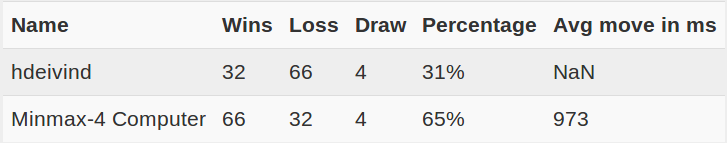
\includegraphics[width=19cm]{thaffe100.png}
\caption{The result of a online fight}
\label{figure4}

\end{figure}


  \begin{tabular}{| l  l  r l |}
    \hline
 	Player 1 & (Our) & wins: & 2 \\
 	Player 2 & (Thaffe) & wins: & 7 \\
 	& &  Ties: & 1 \\
    \hline
  \end{tabular}

\subsubsection{Our vs Victor}

\subsubsection{Our vs Simon \& Håkon}

\subsection{Experience}
Luckily for us, the tournament protocol was pretty straight forward. We got an email giving us the zip file with the needed file(s). The zip had 2 jar files (which had the needed library to connect to the server) and an interface which we needed to implement. There were also an example file which showed us which method we needed to implement and how it was done. \\
It was pretty easy to connect to the server and start playing against the other bots, however the server didn't check for validity (for instance if the move or the given piece is a legal one which meant we had to check for ourselves), this did cause a lot of frustration because the board we were playing on could easily be different from the one on the server. \\
The first thing we noticed when we read the code was that the order of the pieces was different than ours.\\
Their pieces were organized like this:
\begin{verbatim}
(r) (r*) (R) (R*) |r| |r*| |R| |R*| (b) (b*) (B) (B*) |b| |b*| |B| |B*|
\end{verbatim}
and ours were:
\begin{verbatim}
0:|R*|  1:|R|  2: |r*|  3: |r|  4: (R*)  5: (R)  6: (r*)  7: (r)
8:|B*|  9:|B|  10:|b*|  11:|b|  12:(B*)  13:(B)  14:(b*)  15:(b)
\end{verbatim}
but we fixed this easily by tweaking how our pieces were generated, so now our list looks exactly like the protocol's and we can easily receive and send piece index without worrying about which piece is which, because it's the same piece.\\ \\
There's also a bit of frustration involved with the debugging, as the conversion between input/output from java, and javascript with json, proved to be quite a handful. There were also some conflicts regarding who was supposed to start, as the broadcasted player turn sometimes did not add up between our game sessions. We seem to have found the source of the problem but a rare bug did appear from time to time. The first player are supposed to send positionIndex = -1 (which mean that you put down a piece outside the board) and a pieceIndex. However due to the meteor framework (which is what Thaffe's server is running) only sends changes it sometime didn't send a positionIndex = -1, but it sent positionIndex = 0 (this was interpreted wrongly by our client because our client thought it was supposed to start by giving a piece) so when our client got the positionIndex = 0 and a piece X it started by putting the piece it thought it gave to the server on spot 0. Long story short, our client would crash when we got the piece from the server that our client thought it gave in the beginning or the server put down a piece on spot 0 (which was occupied by the first piece on our client's board) this lead to us having 2 different boards on the client and the server side.\\ 
However the bug seems to be fixed, and the problem that we had doesn't always occur, so we can easily just start a new game if a match has crashed. \\ \\
We would like to give credit to Thaffe for writing the protocol, he wrote his code in javascript using the meteor framework, but he was kind enough to write a java protocol and interface so that we could easily connect to his server, and he was also bug fixing and debugging the code when things went wrong. Big kudos to him.


\end{document}